\chapter{系统的测试与评价}

\section{不同虚拟化方案对负载性能影响的比较}

在本节,首先介绍 Tsinghua NOVA 项目中的基准测试套件 Omegabench ,然后通过在不同的
虚拟化平台上运行同样的模仿真实环境的负载,对不同虚拟化方案的效果和实用性作出评估。

\subsection{实验环境}

实验使用的硬件是一台清华同方“超强”系列的塔式服务器,型号是 TP-240 。具体配置如下:

\begin{lstlisting}
Tsinghua-Tongfang TP-240 tower server
    |-- Dual Intel Xeon E5606 @ 2.13 GHz
    |-- 32 GB DDR3 ECC memory
    |-- WDC WD10EALX-229
\end{lstlisting}

宿主机使用的操作系统是 CentOS 7.2 ,也就是目前最新的版本。相应的软件栈也在实验之前更新
到 Red Hat EPEL 软件仓库中的最新版本。

\subsection{负载类型的选择}

常见的基准测试软件可以按照负载类型分成两类。一种是运行理想化的负载,例如计算圆周率的
SuperPI 。在实际应用中,恐怕没有用户会每天使用计算机无穷无尽地计算圆周率,所以这种
负载只能说是对真实世界的计算问题的一种简单的抽象。另一种是运行现实中真实存在的综合性
的计算需求,比如 SPEC CPU 基准测试,包括了许多科学计算任务——流体力学计算、声音识别
等等,又比如 GeekBench ,套件中包含了图象压缩、数据加密、哈希计算等多种个人用户常用的
计算功能的性能评估。

本测试套件 Omegabench 主要是面向大型服务器集群,尤其是虚拟化集群。在本测试套件中,
主要包含了以下几种类型的负载:

\begin{enumerate}
    \item web 服务器:主要包括传统的 HTTP 服务器 Apache httpd 和轻量级
    的 HTTP 服务 mongoose 两个测试项目。基准测试使用的客户端是 Apache 自带的测试程序,
    适用于几乎所有的 HTTP 服务。主要测试指标是服务器的相应速度和吞吐量;
    \item 存储和数据库服务:这个类别包括三个功能互不相同的服务。一是 memcached
    ,一个通用的分布式数据内存缓存 (memory caching) 服务,二是 redis ,一个内存数据存储
    服务,既可以作为缓存 (caching) 也可以作为一个内存数据库,三是 mysql ,一个著名的
    数据库服务;
    \item 压缩和加密:这个类别目前只包含一个测试项目,也就是 xz 的解压缩以及
    tar 解包的综合测试。这个测试既考验 CPU 性能也考验磁盘 I/O 性能。
\end{enumerate}

\subsection{资源限制}

在这一小节,我们说明本次实验对于 LXC 与 KVM 两种虚拟化平台的配置是公平的。

\subsubsection{通过 cgroup 对 LXC 做资源限制}

在 LXC 虚拟容器中,我们通过修改容器的配置文件来对其进行内存的配额限制。在
~\ref{subsubsec:cgroup}小节提到过,现代的 Linux 内核可以通过 cgroup 进行进程组的资源
调配,所以在这里,我们就要修改 cgroup 的相关参数。

以名为 test-fedora-1 的容器举例,修改配置文件,添加:

\begin{lstlisting}
# limit memory
lxc.cgroup.memory.limit_in_bytes = 8G
lxc.cgroup.memory.memsw.limit_in_bytes = 10G
\end{lstlisting}

就可以将总内存限制为 8GB ,内存加 swap 限制为 10GB 。配置文件修改后的 LXC 容器启动日志
如下\footnote{日志较长,这里只提取了关键信息}:

\begin{lstlisting}
cgfs.c:do_setup_cgroup_limits:1922 - cgroup 'devices.allow' set to 'c 5:2 rwm'
cgfs.c:do_setup_cgroup_limits:1922 - cgroup 'memory.limit_in_bytes' set to '8G'
cgfs.c:do_setup_cgroup_limits:1922 - cgroup 'memory.memsw.limit_in_bytes' set to '10G'
cgfs.c:do_setup_cgroup_limits:1926 - cgroup has been setup
\end{lstlisting}

也可以从文件中读取。注意因为 /proc/meminfo 没有对 cgroup 进行过优化,所以它读出来的
内存信息是宿主机的总内存容量而不是容器内部限制使用的配额:

\begin{lstlisting}
[root@test-fedora-1 ~]# cat /sys/fs/cgroup/memory/lxc/test-fedora-1/memory.limit_in_bytes
8589934592
[root@test-fedora-1 ~]# cat /sys/fs/cgroup/memory/lxc/test-fedora-1/memory.memsw.limit_in_bytes
10737418240
\end{lstlisting}

可见,此时该虚拟容器 test-fedora-1 的内存资源已得到了限制。

使用类似的方法可以对 CPU 数量等关键参数进行设置。在本次实验中,因为 LXC 与 KVM 的性能测试是
先后而不是同时运行,所以二者的设置都是使用宿主机全部的 CPU 个数。

\subsubsection{对 QEMU-KVM 进行资源限制}

KVM 有数量众多的前端工具,比如命令行的 virsh (Virtual Shell) 和图形界面的 virt-manager
。我们使用 Red Hat 自家的 GNOME Boxes 作为前端来配置 KVM 的客户虚拟机,这也是 RHEL/CentOS
的默认方案。

\begin{figure}[t]
    \centering
    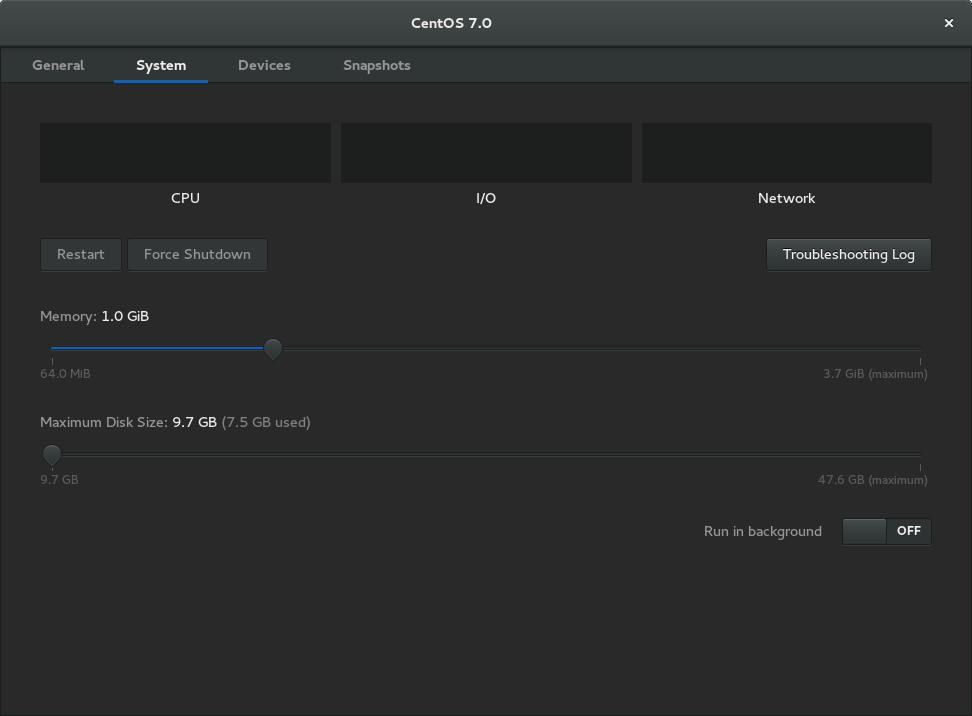
\includegraphics[width=0.7\textwidth]{gnome-boxes-config}
    \caption{通过 GNOME Boxes 配置客户虚拟机}
    \label{fig:gnome-boxes-config}
\end{figure}

如图~\ref{fig:gnome-boxes-config}所示,通过图形界面能简单地配置内存和处理器的配额。
通过 virsh dominfo 命令可以进行查看:

\begin{lstlisting}
$ virsh dominfo fedora22-wor
Id:             3
Name:           fedora22-wor
UUID:           3fe3e047-aa2e-4280-90d4-97c0816e3529
OS Type:        hvm
State:          running
CPU(s):         8
CPU time:       305743.4s
Max memory:     8373248 KiB
Used memory:    8373184 KiB
Persistent:     yes
Autostart:      disable
Managed save:   no
Security model: selinux
Security DOI:   0
Security label: unconfined_u:unconfined_r:svirt_t:s0:c355,c485 (enforcing)
\end{lstlisting}

\subsection{运行本测试套件}

我们的测试套件的远端仓库 (repository) 托管在 GitHub 上,使用 git 进行版本控制。可以
以源代码的形式获得这个套件。

\subsubsection{目录结构}

工程的根目录包含一个叫 tests/ 的目录,和其它若干个以测试用例的名称命名的目录,比如 mongoose/
和 redis/ 等。tests/ 目录包含了全部测试脚本,和测试使用的配置文件,还有以表格或者图表的形式
收集测试结果的相关代码。而以测试项目命名的目录中一般有一个用于自动下载和编译安装测试用的服务
的脚本,还有一个开启服务器的脚本。通过先后运行这两个脚本可以完成测试用服务的自动部署和配置。
还有一个文件保存编译的时候使用的配置信息,比如服务器软件的版本、所需依赖的版本等。

\subsubsection{安装依赖和编译测试服务}

以 Apache httpd 为例,首先通过保管理器安装相关的依赖:

\begin{lstlisting}[language=bash]
dnf install tar wget # required when using Fedora mininal installation
dnf install gcc make
dnf install pcre-devel
dnf install libxml2-devel
dnf install xz       # for testing xz and tar
\end{lstlisting}

然后需要在相应的 shell 配置文件比如 .bashrc 中定义 \$OMEGA\_HOME 这个变量:

\begin{lstlisting}[language=bash]
export OMEGA_HOME="your/preferred/dir/here"
\end{lstlisting}

然后运行叫做 \$OMEGA\_HOME/apache-httpd/download-compile-apache.sh 即可自动完成
httpd 以及 PHP 解释器的编译安装,而且会自动生成一个测试用的配置文件 httpd.conf 。使用
apachectl 可以控制 httpd 的运行与停止,通过 -f 参数可以指定配置文件。

\subsubsection{运行测试程序}

仍然以 Apache httpd 举例,通过运行 run-ab-tests.py 可以自动进行基准测试并以列表和
柱状图的形式显示出性能数据。

相应的测试程序配置文件是 ab-tests-config.json ,一个简单的测试本机的例子如下:

\begin{lstlisting}
{
  "ab": "$OMEGA_HOME/apache-httpd/install/bin/ab",
  "num_req": 128,
  "concurrency": 8,
  "port": 7000,
  "ip_addr": [
    "127.0.0.1"
  ]
}
\end{lstlisting}

在这个例子中,测试客户端一共向服务器发送 128 个 HTTP 请求 (requests) ,
并发度 (concurreny level) 是 8 ,连接到服务器的 7000 端口,服务器的 IP 地址是
127.0.0.1 。

\subsection{实验结果}

\subsubsection{Web 服务器}

Mongoose 和 Apache httpd 的测试结果分别如表~\ref{tab:mongoose-perf}
以及~\ref{tab:apache-perf}。

\begin{table}[H]
    \centering
    \caption{Mongoose 的性能测试结果}
    \begin{tabular}{||c c c c||}
        \hline
        FIELD & KVM & LXC & BAREMETAL \\
        \hline
        \hline
        Time per request (ms) & 255.608 & 267.923 & 284.447 \\
        \hline
        Requests per sec & 31.3 & 29.86 & 28.12 \\
        \hline
        Transfer rate (KB/s) & 3.39 & 3.24 & 3.05 \\
        \hline
        Time taken (s) & 4.09 & 4.287 & 4.551 \\
        \hline
    \end{tabular}
    \label{tab:mongoose-perf}
\end{table}

\begin{table}[H]
    \centering
    \caption{Apache httpd 的性能测试结果}
    \begin{tabular}{||c c c c||}
        \hline
        FIELD & KVM & LXC & BAREMETAL \\
        \hline
        \hline
        Time per request (ms) & 275.432 & 253.109 & 271.302 \\
        \hline
        Requests per sec & 29.05 & 31.61 & 29.49 \\
        \hline
        Transfer rate (KB/s) & 6.44 & 7.01 & 6.54 \\
        \hline
        Time taken (s) & 4.407 & 4.05 & 4.341 \\
        \hline
    \end{tabular}
    \label{tab:apache-perf}
\end{table}

\subsubsection{存储和数据库服务}

Memcached、Redis 还有 Mysql 的测试情况分别如表~\ref{tab:memcached-perf}、
~\ref{tab:redis-perf}还有~\ref{tab:mysql-perf}所示:

\begin{table}[H]
    \centering
    \caption{Memcached 的性能测试结果}
    \begin{tabular}{||c c c c||}
        \hline
        FIELD & KVM & LXC & BAREMETAL \\
        \hline
        \hline
        Total time (s) & 4.685 & 1.707 & 1.292 \\
        \hline
    \end{tabular}
    \label{tab:memcached-perf}
\end{table}

\begin{table}[H]
    \centering
    \caption{Redis 的性能测试结果}
    \begin{tabular}{||c c c c||}
        \hline
        FIELD (req/s) & KVM & LXC & BAREMETAL \\
        \hline
        \hline
        PING\_INLINE & 25859.84 & 44365.57 & 49261.09 \\
        \hline
        PING\_BULK & 31113.88 & 44208.66 & 50968.40 \\
        \hline
        SET & 26096.03 & 48030.74 & 59594.76 \\
        \hline
        GET & 28003.36 & 54171.18 & 55834.73 \\
        \hline
        INCR & 25284.45 & 46750.82 & 58788.95 \\
        \hline
        LPUSH & 26961.44 & 48123.20 & 60240.96 \\
        \hline
        RPUSH & 27300.03 & 46750.82 & 59952.04 \\
        \hline
        LPOP & 23337.22 & 46339.20 & 60024.01 \\
        \hline
        RPOP & 26198.59 & 46533.27 & 59523.81 \\
        \hline
        SADD & 26075.62 & 46360.68 & 58685.45 \\
        \hline
        SPOP & 26253.61 & 46794.57 & 57240.98 \\
        \hline
        LRANGE\_100 & 28232.64 & 28320.59 & 29868.58 \\
        \hline
        LRANGE\_300 & 12992.08 & 10736.53 & 12729.12 \\
        \hline
        LRANGE\_500 & 9095.04 & 8318.78 & 9489.47 \\
        \hline
        LRANGE\_600 & 7808.23 & 7190.62 & 7487.27 \\
        \hline
        MSET (10 keys) & 23691.07 & 42936.88 & 57903.88 \\
        \hline
    \end{tabular}
    \label{tab:redis-perf}
\end{table}

\begin{table}[H]
    \centering
    \caption{Mysql 的性能测试结果}
    \begin{tabular}{||c c c c||}
        \hline
        FIELD & KVM & LXC & BAREMETAL \\
        \hline
        \hline
        Total time (s) & 4.2884 & 4.0552 & 3.9215 \\
        \hline
        Response time (ms) & 336.99 & 315.09 & 307.25 \\
        \hline
    \end{tabular}
    \label{tab:mysql-perf}
\end{table}

\subsubsection{解压缩}

tar/xz 的测试结果如表~\ref{tab:tar-xz-perf}所示:

\begin{table}[H]
    \centering
    \caption{Tar/xz 的性能测试结果}
    \begin{tabular}{||c c c c||}
        \hline
        FIELD & KVM & LXC & BAREMETAL \\
        \hline
        \hline
        Real (s) & 17.901 & 26.646 & 16.518 \\
        \hline
        User (s) & 11.331 & 11.065 & 11.025 \\
        \hline
        Sys (s) & 6.106 & 5.857 & 5.477 \\
        \hline
    \end{tabular}
    \label{tab:tar-xz-perf}
\end{table}

\subsection{小结}

在上述几个实验中,除了 Mongoose 和 Tar/xz 两项,LXC 都相较于 QEMU-KVM 有性能优势。
当然,KVM 是虚拟机管理程序中非常高效的一种,它是完全利用硬件虚拟化的。LXC 虚拟容器能
在多数指标上优于 KVM ,证明虚拟容器技术有自己的优势。

\section{调度性能评估}

\subsection{实验环境}

实验环境包含三台由千兆以太网交换机相连的机架式服务器,它们的匹配如下:

\begin{lstlisting}
Dell PowerEdge R720
|-- Dual Xeon E5-2640 v2
|-- 32GB DDR3 ECC SDRAM
|-- CentOS 7.2 x86_64 (Linux 3.10.0)
|-- Oracle Java SE 1.7.0_79
|-- Libvirt 1.2.17
\end{lstlisting}

其中一台作为主节点 (master node) ,另外两台作为从节点 (slave node) 。主节点还作为另外
两者的网关,从节点不运行防火墙,主节点运行 iptables 服务作为防火墙,关闭了 CentOS 默认
使用的 firewalld 。从节点所有 IPV4 流量需要经过主节点转发。

\subsection{迁移开销}

在迁移的实验中,我们使用理想化的负载 toy.py ,它的作用是不断把内存中的一个计数变量写入磁盘
块设备中的文件 testfile ,通过查看 testfile 中的数字可以判断实时迁移 (live migration)
是否成功。

\begin{lstlisting}[language=Python]
#!/usr/bin/python2.7
import time

data = 42

while(True):
    with open("testfile", "w+") as f:
        f.write(str(data) + '\n')
    data += 1
    time.sleep(10)
\end{lstlisting}

通过在 Tsinghua NOVA 系统中打印日志的形式进行测量。一次运行的结果如下:

\begin{lstlisting}
2016-05-05 21:08:43,693: uuid of domain to migrate is 30680a29-215a-48a6-b728-5643fb7d7dc7
2016-05-05 21:08:43,693: checkpoint! container name: testlxc4; process name: toy.py; ip addr: 192.168.122.4
2016-05-05 21:08:43,694: cmd: /home/Nova/lxc-cr-wrapper checkpoint -c testlxc4 -p toy.py -i 192.168.122.4
2016-05-05 21:08:54,009: dst domain created.
2016-05-05 21:08:54,009: restoring process in destination domain...
2016-05-05 21:08:54,009: restore! dst ip: 192.168.7.101; container name: testlxc4; process name: toy.py; ip addr: 192.168.122.4
2016-05-05 21:08:54,010: cmd: ssh 192.168.7.101 /home/Nova/lxc-cr-wrapper restore -c testlxc4 -p toy.py -i 192.168.122.4
2016-05-05 21:09:21,294: restore succeeded!
\end{lstlisting}

可以看出,在源宿主机上的虚拟容器中 checkpoint 负载进程需要大约 10 秒,而在目标宿主机上
迁移过后的虚拟容器中 restore 负载进程需要 27 秒左右。整个过程存在大约 40 秒的开销。

% TODO 在这里测量一下创建虚拟机的开销
% TODO 和 KVM 的作对比
